% Created by tikzDevice version 0.12.3.1 on 2023-10-19 11:54:22
% !TEX encoding = UTF-8 Unicode
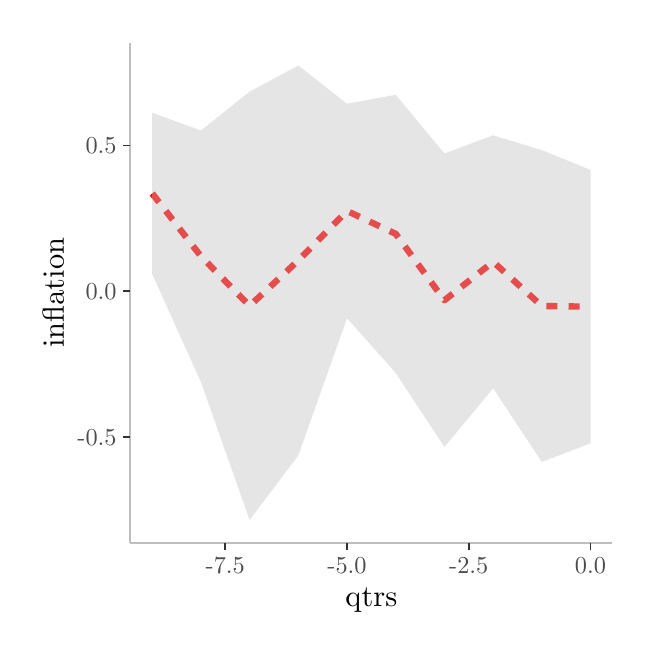
\begin{tikzpicture}[x=1pt,y=1pt]
\definecolor{fillColor}{RGB}{255,255,255}
\path[use as bounding box,fill=fillColor,fill opacity=0.00] (0,0) rectangle (216.81,216.81);
\begin{scope}
\path[clip] (  0.00,  0.00) rectangle (216.81,216.81);
\definecolor{drawColor}{RGB}{255,255,255}
\definecolor{fillColor}{RGB}{255,255,255}

\path[draw=drawColor,line width= 0.6pt,line join=round,line cap=round,fill=fillColor] (  0.00,  0.00) rectangle (216.81,216.81);
\end{scope}
\begin{scope}
\path[clip] ( 37.09, 30.69) rectangle (211.31,211.31);
\definecolor{drawColor}{RGB}{255,255,255}

\path[draw=drawColor,line width= 0.6pt,line join=round] ( 37.09, 68.88) --
	(211.31, 68.88);

\path[draw=drawColor,line width= 0.6pt,line join=round] ( 37.09,121.58) --
	(211.31,121.58);

\path[draw=drawColor,line width= 0.6pt,line join=round] ( 37.09,174.28) --
	(211.31,174.28);

\path[draw=drawColor,line width= 0.6pt,line join=round] ( 71.41, 30.69) --
	( 71.41,211.31);

\path[draw=drawColor,line width= 0.6pt,line join=round] (115.40, 30.69) --
	(115.40,211.31);

\path[draw=drawColor,line width= 0.6pt,line join=round] (159.40, 30.69) --
	(159.40,211.31);

\path[draw=drawColor,line width= 0.6pt,line join=round] (203.39, 30.69) --
	(203.39,211.31);
\definecolor{drawColor}{RGB}{255,0,0}

\path[draw=drawColor,line width= 2.3pt,dash pattern=on 4pt off 4pt ,line join=round] ( 45.01,156.90) --
	( 62.61,134.20) --
	( 80.20,116.30) --
	( 97.80,132.68) --
	(115.40,150.58) --
	(133.00,142.31) --
	(150.60,118.31) --
	(168.19,132.20) --
	(185.79,116.23) --
	(203.39,116.00);
\definecolor{fillColor}{RGB}{190,190,190}

\path[fill=fillColor,fill opacity=0.40] ( 45.01,186.05) --
	( 62.61,179.64) --
	( 80.20,193.70) --
	( 97.80,203.10) --
	(115.40,189.31) --
	(133.00,192.56) --
	(150.60,171.34) --
	(168.19,177.89) --
	(185.79,172.57) --
	(203.39,165.39) --
	(203.39, 66.62) --
	(185.79, 59.89) --
	(168.19, 86.51) --
	(150.60, 65.29) --
	(133.00, 92.06) --
	(115.40,111.84) --
	( 97.80, 62.27) --
	( 80.20, 38.90) --
	( 62.61, 88.76) --
	( 45.01,127.74) --
	cycle;

\path[] ( 45.01,186.05) --
	( 62.61,179.64) --
	( 80.20,193.70) --
	( 97.80,203.10) --
	(115.40,189.31) --
	(133.00,192.56) --
	(150.60,171.34) --
	(168.19,177.89) --
	(185.79,172.57) --
	(203.39,165.39);

\path[] (203.39, 66.62) --
	(185.79, 59.89) --
	(168.19, 86.51) --
	(150.60, 65.29) --
	(133.00, 92.06) --
	(115.40,111.84) --
	( 97.80, 62.27) --
	( 80.20, 38.90) --
	( 62.61, 88.76) --
	( 45.01,127.74);
\end{scope}
\begin{scope}
\path[clip] (  0.00,  0.00) rectangle (216.81,216.81);
\definecolor{drawColor}{RGB}{190,190,190}

\path[draw=drawColor,line width= 0.6pt,line join=round] ( 37.09, 30.69) --
	( 37.09,211.31);
\end{scope}
\begin{scope}
\path[clip] (  0.00,  0.00) rectangle (216.81,216.81);
\definecolor{drawColor}{gray}{0.30}

\node[text=drawColor,anchor=base east,inner sep=0pt, outer sep=0pt, scale=  0.88] at ( 32.14, 65.85) {-0.5};

\node[text=drawColor,anchor=base east,inner sep=0pt, outer sep=0pt, scale=  0.88] at ( 32.14,118.55) {0.0};

\node[text=drawColor,anchor=base east,inner sep=0pt, outer sep=0pt, scale=  0.88] at ( 32.14,171.25) {0.5};
\end{scope}
\begin{scope}
\path[clip] (  0.00,  0.00) rectangle (216.81,216.81);
\definecolor{drawColor}{gray}{0.20}

\path[draw=drawColor,line width= 0.6pt,line join=round] ( 34.34, 68.88) --
	( 37.09, 68.88);

\path[draw=drawColor,line width= 0.6pt,line join=round] ( 34.34,121.58) --
	( 37.09,121.58);

\path[draw=drawColor,line width= 0.6pt,line join=round] ( 34.34,174.28) --
	( 37.09,174.28);
\end{scope}
\begin{scope}
\path[clip] (  0.00,  0.00) rectangle (216.81,216.81);
\definecolor{drawColor}{RGB}{190,190,190}

\path[draw=drawColor,line width= 0.6pt,line join=round] ( 37.09, 30.69) --
	(211.31, 30.69);
\end{scope}
\begin{scope}
\path[clip] (  0.00,  0.00) rectangle (216.81,216.81);
\definecolor{drawColor}{gray}{0.20}

\path[draw=drawColor,line width= 0.6pt,line join=round] ( 71.41, 27.94) --
	( 71.41, 30.69);

\path[draw=drawColor,line width= 0.6pt,line join=round] (115.40, 27.94) --
	(115.40, 30.69);

\path[draw=drawColor,line width= 0.6pt,line join=round] (159.40, 27.94) --
	(159.40, 30.69);

\path[draw=drawColor,line width= 0.6pt,line join=round] (203.39, 27.94) --
	(203.39, 30.69);
\end{scope}
\begin{scope}
\path[clip] (  0.00,  0.00) rectangle (216.81,216.81);
\definecolor{drawColor}{gray}{0.30}

\node[text=drawColor,anchor=base,inner sep=0pt, outer sep=0pt, scale=  0.88] at ( 71.41, 19.68) {-7.5};

\node[text=drawColor,anchor=base,inner sep=0pt, outer sep=0pt, scale=  0.88] at (115.40, 19.68) {-5.0};

\node[text=drawColor,anchor=base,inner sep=0pt, outer sep=0pt, scale=  0.88] at (159.40, 19.68) {-2.5};

\node[text=drawColor,anchor=base,inner sep=0pt, outer sep=0pt, scale=  0.88] at (203.39, 19.68) {0.0};
\end{scope}
\begin{scope}
\path[clip] (  0.00,  0.00) rectangle (216.81,216.81);
\definecolor{drawColor}{RGB}{0,0,0}

\node[text=drawColor,anchor=base,inner sep=0pt, outer sep=0pt, scale=  1.10] at (124.20,  7.64) {qtrs};
\end{scope}
\begin{scope}
\path[clip] (  0.00,  0.00) rectangle (216.81,216.81);
\definecolor{drawColor}{RGB}{0,0,0}

\node[text=drawColor,rotate= 90.00,anchor=base,inner sep=0pt, outer sep=0pt, scale=  1.10] at ( 13.08,121.00) {inflation};
\end{scope}
\end{tikzpicture}
